%%
%% Automatically generated file from DocOnce source
%% (https://github.com/hplgit/doconce/)
%%
%%


%-------------------- begin preamble ----------------------

\documentclass[%
oneside,                 % oneside: electronic viewing, twoside: printing
final,                   % draft: marks overfull hboxes, figures with paths
10pt]{article}

\listfiles               %  print all files needed to compile this document

\usepackage{relsize,makeidx,color,setspace,amsmath,amsfonts,amssymb}
\usepackage[table]{xcolor}
\usepackage{bm,ltablex,microtype}

\usepackage[pdftex]{graphicx}

\usepackage[T1]{fontenc}
%\usepackage[latin1]{inputenc}
\usepackage{ucs}
\usepackage[utf8x]{inputenc}

\usepackage{lmodern}         % Latin Modern fonts derived from Computer Modern

% Hyperlinks in PDF:
\definecolor{linkcolor}{rgb}{0,0,0.4}
\usepackage{hyperref}
\hypersetup{
    breaklinks=true,
    colorlinks=true,
    linkcolor=linkcolor,
    urlcolor=linkcolor,
    citecolor=black,
    filecolor=black,
    %filecolor=blue,
    pdfmenubar=true,
    pdftoolbar=true,
    bookmarksdepth=3   % Uncomment (and tweak) for PDF bookmarks with more levels than the TOC
    }
%\hyperbaseurl{}   % hyperlinks are relative to this root

\setcounter{tocdepth}{2}  % levels in table of contents

% Tricks for having figures close to where they are defined:
% 1. define less restrictive rules for where to put figures
\setcounter{topnumber}{2}
\setcounter{bottomnumber}{2}
\setcounter{totalnumber}{4}
\renewcommand{\topfraction}{0.95}
\renewcommand{\bottomfraction}{0.95}
\renewcommand{\textfraction}{0}
\renewcommand{\floatpagefraction}{0.75}
% floatpagefraction must always be less than topfraction!
% 2. ensure all figures are flushed before next section
\usepackage[section]{placeins}
% 3. enable begin{figure}[H] (often leads to ugly pagebreaks)
%\usepackage{float}\restylefloat{figure}

\usepackage[framemethod=TikZ]{mdframed}

% --- begin definitions of admonition environments ---

% --- end of definitions of admonition environments ---

% prevent orhpans and widows
\clubpenalty = 10000
\widowpenalty = 10000

% --- end of standard preamble for documents ---


% insert custom LaTeX commands...

\raggedbottom
\makeindex
\usepackage[totoc]{idxlayout}   % for index in the toc
\usepackage[nottoc]{tocbibind}  % for references/bibliography in the toc

%-------------------- end preamble ----------------------

\begin{document}

% matching end for #ifdef PREAMBLE

\newcommand{\exercisesection}[1]{\subsection*{#1}}


% ------------------- main content ----------------------



% ----------------- title -------------------------

\thispagestyle{empty}

\begin{center}
{\LARGE\bf
\begin{spacing}{1.25}
Master program in Computational Science  at the University of Oslo
\end{spacing}
}
\end{center}

% ----------------- author(s) -------------------------

\begin{center}
{\bf Welcome to all of you${}^{}$} \\ [0mm]
\end{center}

\begin{center}
% List of all institutions:
\end{center}
    
% ----------------- end author(s) -------------------------


% --- begin date ---
\begin{center}
August 14, 2018
\end{center}
% --- end date ---

\vspace{1cm}


% !split
\subsection*{Where do I find these slides?}


% --- begin paragraph admon ---
\paragraph{}
Go to \href{{http://mhjensen.github.io/CPMLS/doc/pub/Welcome/html/Welcome-bs.html}}{\nolinkurl{http://mhjensen.github.io/CPMLS/doc/pub/Welcome/html/Welcome-bs.html}}

As soon as we have a complete mailing list, we will send the links electronically to you, with weekly updates about the program as well.
% --- end paragraph admon ---



% !split
\subsection*{The coming job market needs people with your background!}

% --- begin paragraph admon ---
\paragraph{}
The \href{{https://www.mckinsey.com/business-functions/mckinsey-analytics/our-insights/the-age-of-analytics-competing-in-a-data-driven-world}}{consulting company McKinsey recently released a report} arguing that the need for computational and data scientists – that is,
workers who can successfully analyze, model, and interpret data, and use it to inform critical business
decisions - is going to grow rapidly. A wide range of industries now use computational
modeling and data analytics to inform many aspects of their day-to-day practices, encompassing
a range of activities that include product design, optimizing manufacturing processes, hiring decisions,
and choosing advertising targets. The trend is clear, as are the implications for new employees
– being fluent in the tools used to work with data and computational models, as well as to be
intelligent consumers of the products of these tools, will be a critical and high-demand skillset.
% --- end paragraph admon ---



% !split
\subsection*{Why should we focus on Computational Science and Data Science?}

% --- begin paragraph admon ---
\paragraph{}
\begin{itemize}
\item \href{{http://pathways.acm.org/executive-summary.html}}{By 2020, it is expected that one of every two jobs in the STEM fields will be in computing} (Association for Computing Machinery, 2013)

\item Computation is an essential and cross-cutting element of all S(cience)T(echnology)E(ngineering)M(mathematics) disciplines

\item Computational science has developed into a discipline of its own right

\item Computations and the understanding of large data sets will play an even larger role in basically all disciplines of STEM fields, Medicine, the Social Sciences, the Humanities and  education

\item Students at both undergraduate and graduate level are unprepared to use computational modeling, data science, and high performance computing – skills valued by a very broad range of employers.

\item The 3rd Industrial Revolution will alter significantly the demands on the workforce. To adapt a highly-qualified workforce to coming challenges  requires strong fundamental bases in STEM fields. Computational Science can provide such a background at all stages.
\end{itemize}

\noindent
% --- end paragraph admon ---




% !split
\subsection*{Master program in Computational Science}

% --- begin paragraph admon ---
\paragraph{}

The program is a collaboration between seven departments and classical disciplines:

\begin{itemize}
 \item Institute of Theoretical Astrophysics

 \item Department of Biosciences

 \item Department of Chemistry

 \item Department of Geoscience

 \item Department of Informatics

 \item Department of Mathematics

 \item Department of Physics
\end{itemize}

\noindent
The program is multidisciplinary and everbody who  has completed
undergraduate studies in science and engineering, with a sufficient
quantitative background, is eligible.  The language of instruction is
Norwegian or English.
% --- end paragraph admon ---





% !split
\subsection*{Strategic importance}

The program will educate the next generation of cross-disciplinary
science students with the knowledge, skills, and values needed to pose
and solve current and new scientific, technological and societal
challenges. The program will lay the foundation for cross-disciplinary
educational, research and innovation activities.

It is the first educational program to
comprehensively treat computation as the \emph{triple junction} of
algorithm development and analysis, high performance computing, and
applications to scientific and engineering modeling and data
science. This approach recognizes computation as a new discipline
rather than being decentralized into isolated sub-disciplines. The CS program
will  will enable application-driven computational modeling
while also exposing disciplinary computational scientists to
advanced tools and techniques, which will ignite new
transformational connections in research and education.




\vspace{6mm}

% inline figure
\centerline{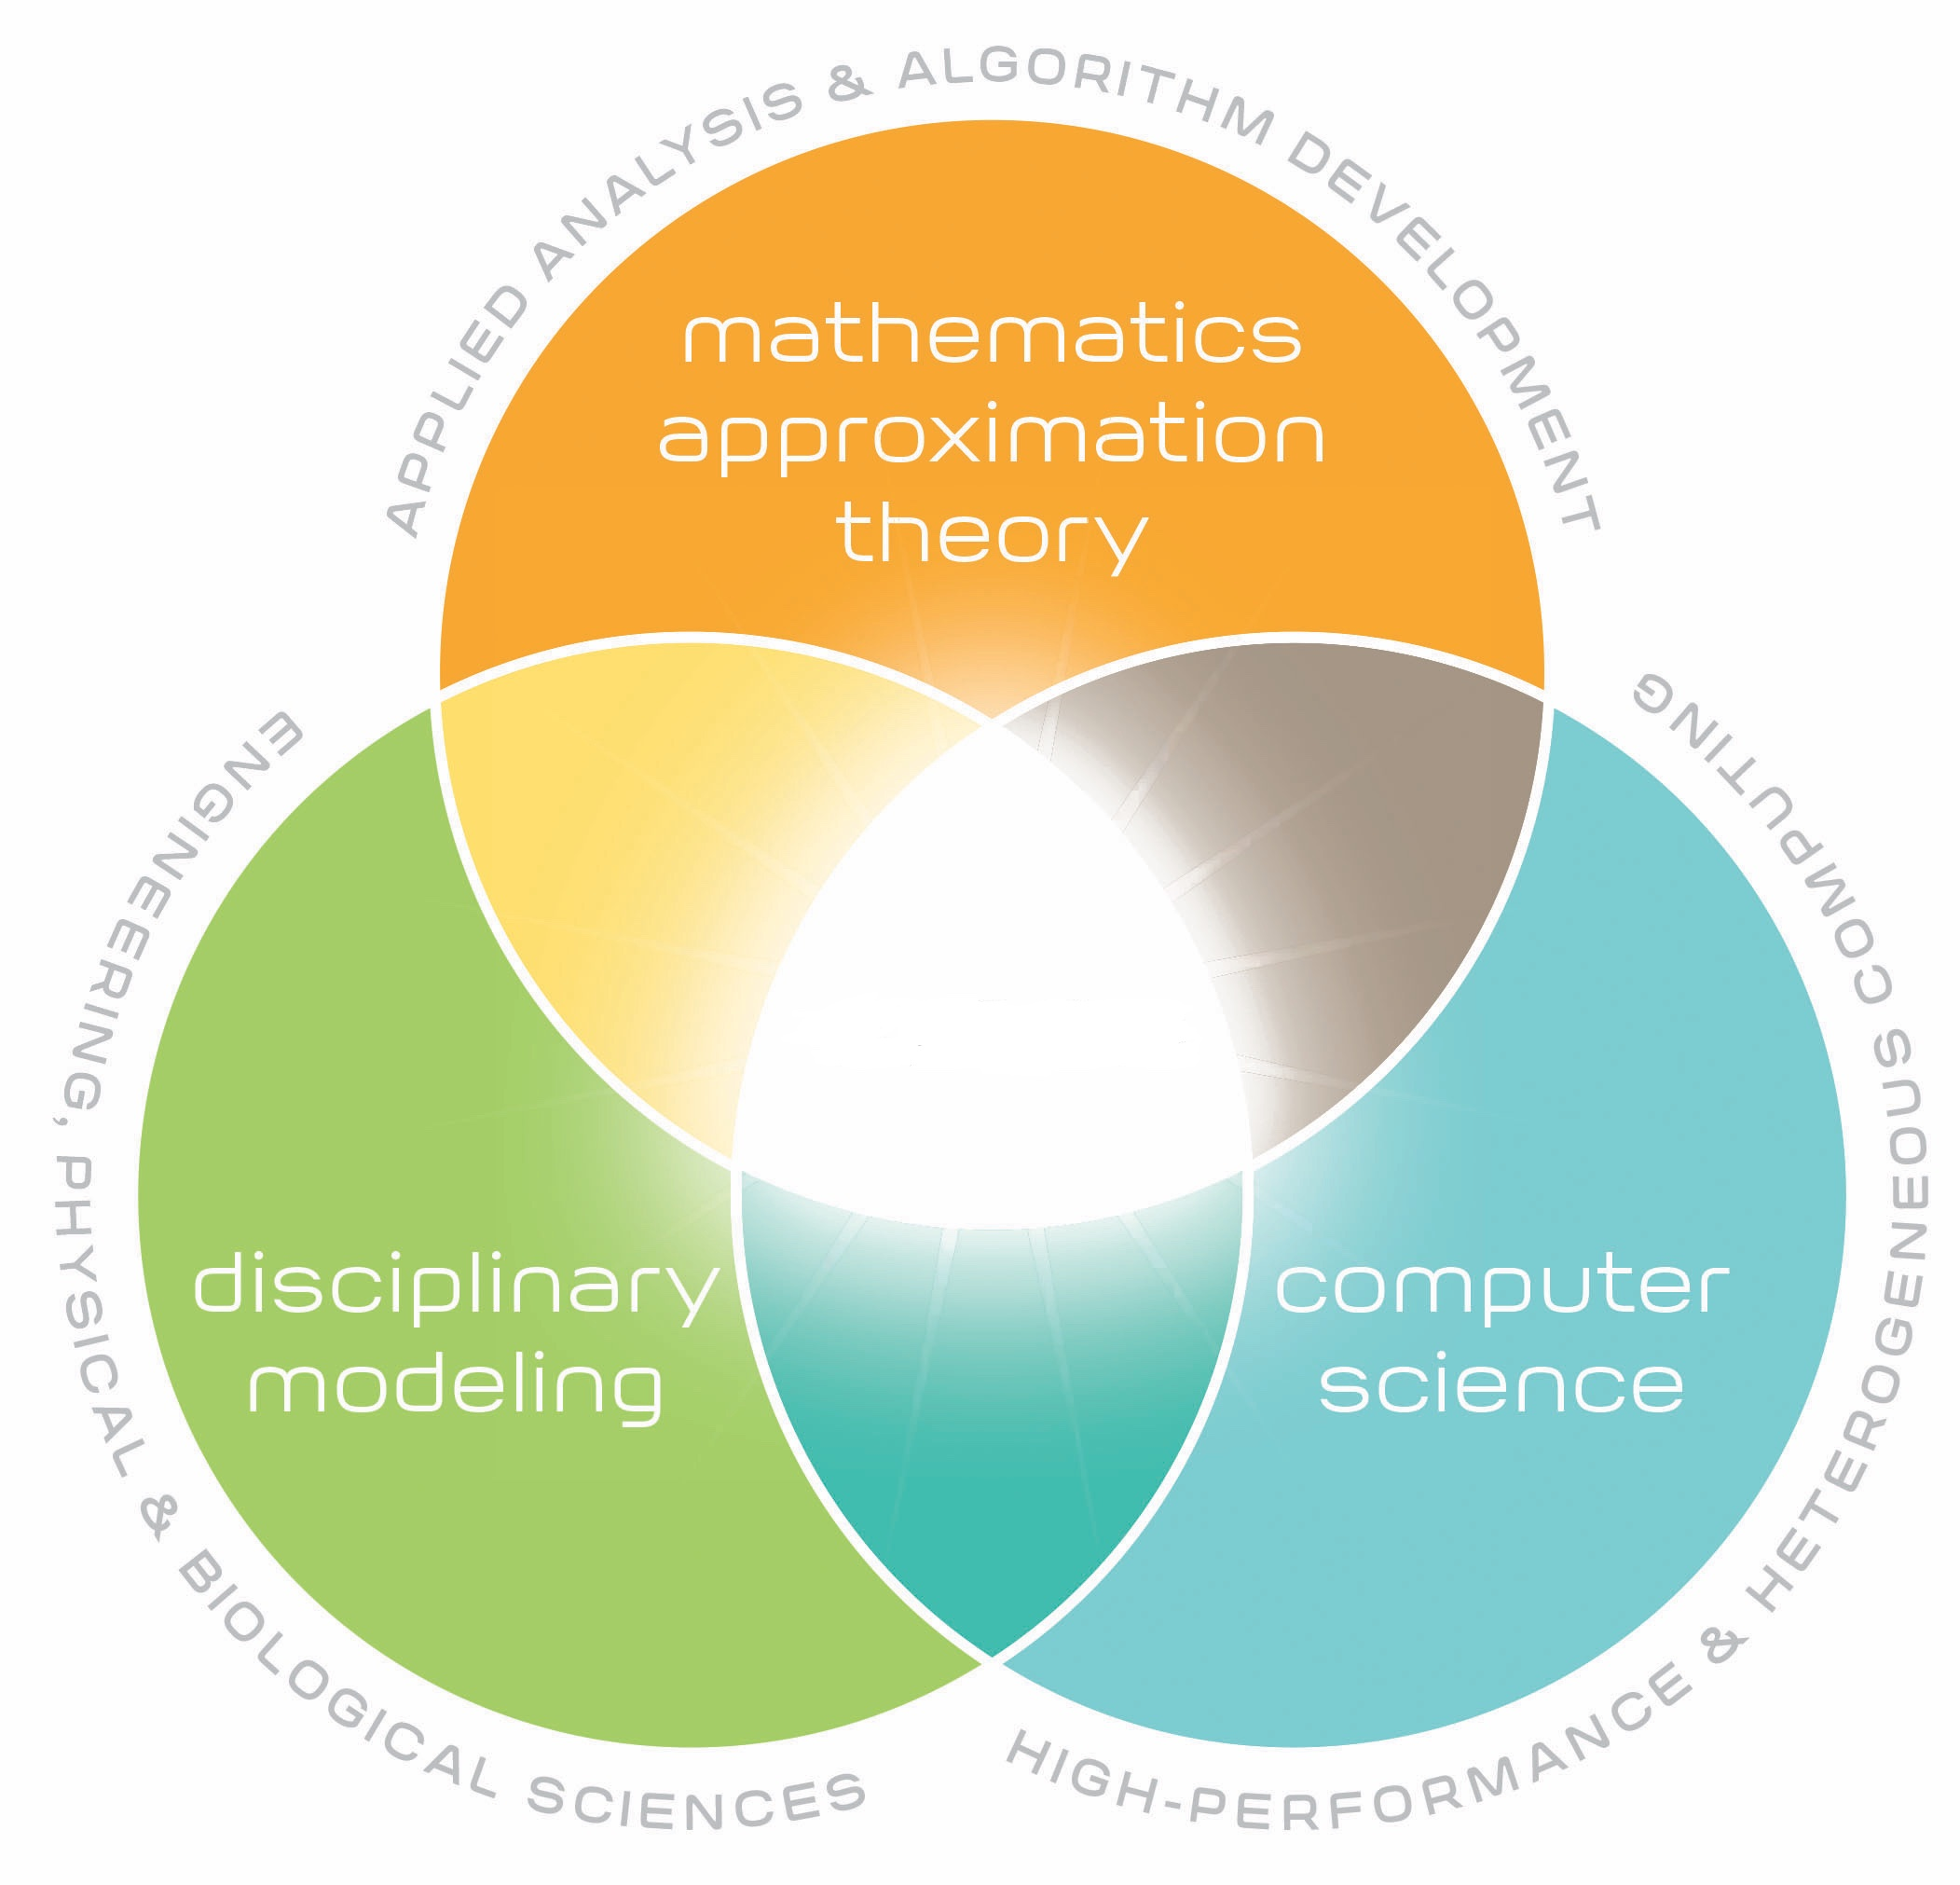
\includegraphics[width=0.6\linewidth]{figslides/cs.jpg}}

\vspace{6mm}




% !split
\subsection*{Vision for the future: Scientific Computing and Data Science}

Scientific computing focuses on the development of predictive computer
models of the world around us. As study of physical phenomena through
experimentation has become impossible, impractical and/or expensive,
computational modeling has become the primary tool for
understanding—equal in stature to analysis and experiment. 
The discipline of scientific computing
is the development of new methods that make challenging problems
tractable on modern computing platforms, providing scientists and
engineers with key windows into the world around us.

Data science focuses on the development of tools designed to find
trends within datasets that help scientists who are challenged with
massive amounts of data to assess key relations within those
datasets. These key relations provide hooks that allow scientists to
identify models which, in turn, facilitate making accurate predictions
in complex systems. For example, a key data science goal on the
biological side would be better care for patients (e.g., personalized
medicine). Given a patient’s genetic makeup, the proper data-driven
model would identify the most effective treatment for that patient.


% !split
\subsection*{Aims of the program}


A specific aim of this program is to develop your ability to pose and
solve problems that combine  insights from a specific discipline with mathematical tools
and computational skills. This provides a unique combination
of applied and theoretical knowledge and skills. These features are invaluable
for the development of multi-disciplinary educational and research programs.
The main focus is not to educate computer
specialists, but to educate students with a solid understanding in basic science
as well as an integrated knowledge on how  to use
essential methods from computational science. This requires an
education that covers both the specific disciplines like physics, biology,
geoscience, mathematics etc with a strong background in computational science.


A significant aspect of this program is the ability to offer new educational
opportunities that are aligned with the needs of a 21st century
workforce. Many companies are seeking
individuals who have knowledge of both a specific discipline and
computational modeling.


% !split
\subsection*{Scientific and educational motivation}


% --- begin paragraph admon ---
\paragraph{Applications of simulation.}
Numerical simulations of various systems in science are central to our
basic understanding of nature and technlogy.
The increase in computational power,
improved algorithms for solving problems in science as well as access
to high-performance facilities, allow researchers nowadays to study
complicated systems across many length and energy scales. Applications
span from studying quantum physical systems in nanotechnology and the
characteristics of new materials or subamotic physics at its smallest
length scale, to simulating galaxies and the evolution of the universe.
In between, simulations are key to understanding
cancer treatment and how the brain works,
predicting climate changes and this week's weather,
simulating natural disasters, semi-conductor devices,
quantum computers, as well as assessing risk in the insurance and
financial industry. These are just a few topics
already well covered at the University of Oslo and that can be
topics for coming thesis projects as well as research directions.
% --- end paragraph admon ---




% !split
\subsection*{Multiscale modeling is a big open research question}



% --- begin paragraph admon ---
\paragraph{}
Today's problems, unlike traditional
science and engineering, involve complex systems with many distinct
physical processes. The wide open research topic of this century, both
in industry and at universities, is how to effectively couple
processes across different length and energy scales. Progress will
rely on a multi-disciplinary approach and therefore a need for
a multi-disciplinary educational program.
% --- end paragraph admon ---




% --- begin paragraph admon ---
\paragraph{}
The CS program aims at giving you  the right
multi-disciplinary background and computational thinking for
understanding today's simulation technology and its challenges.
% --- end paragraph admon ---







% !split
\subsection*{Computing competence}

% --- begin paragraph admon ---
\paragraph{}
Computing means solving scientific problems using computers. It covers
numerical as well as symbolic computing. Computing is also about
developing an understanding of the scientific process by enhancing
algorithmic thinking when solving problems.  Computing competence has
always been a central part of the science and engineering
education.

Modern computing competence is about

\begin{itemize}
\item derivation, verification, and implementation of algorithms

\item understanding what can go wrong with algorithms

\item overview of important, known algorithms

\item understanding how algorithms are used to solve mathematical problems

\item reproducible science and ethics

\item algorithmic thinking for gaining deeper insights about scientific problems
\end{itemize}

\noindent
% --- end paragraph admon ---




% !split
\subsection*{Key elements in computing competence}

% --- begin paragraph admon ---
\paragraph{}
The power of the scientific method lies in identifying a given problem
as a special case of an abstract class of problems, identifying
general solution methods for this class of problems, and applying a
general method to the specific problem (applying means, in the case of
computing, calculations by pen and paper, symbolic computing, or
numerical computing by ready-made and/or self-written software). This
generic view on problems and methods is particularly important for
understanding how to apply available, generic software to solve a
particular problem.


Computing competence represents a central element
in scientific problem solving, from basic education and research to
essentially almost all advanced problems in modern
societies. Computing competence is simply central to further
progress. It enlarges the body of tools available to students and
scientists beyond classical tools and allows for a more generic
handling of problems. Focusing on algorithmic aspects results in
deeper insights about scientific problems.
% --- end paragraph admon ---



% !split
\subsection*{Overarching description of the CS program}

% --- begin paragraph admon ---
\paragraph{}
In this program you learn to use the computer as a laboratory for
solving problems in science and engineering. The program offers
exciting thesis projects from many disciplines: biology and life
science, chemistry, mathematics, informatics, physics, geophysics,
mechanics, geology, computational finance, computational informatics, b
ig data analysis, digital signal processing
and image analysis – you select research field according to
your interests.

A Master’s degree from this program gives you a methodical
training in planning, conducting, and reporting large research
projects, often together with other students and university teachers.
The projects emphasize finding practical solutions, developing an
intuitive understanding of the science and the scientific methods
needed to solve complicated problems, use of many tools, and not least
developing own creativity and independent thinking. The thesis
work is a scientific project where you learn to tackle a
scientific problem in a professional manner.   The program aims also at
developing a deep understanding of the role of computing in solving modern scientific
problems. 

From this program you gain  deep insights in the fundamnetal role
computations play  in our advancement of science and technology, as well as the role computations play  in society.
% --- end paragraph admon ---



% !split
\subsection*{The program opens up for flexible backgrounds}


% --- begin paragraph admon ---
\paragraph{}
While discipline-based master's programs tend to introduce very strict
requirements to courses, we believe in adapting a computational thesis
topic to the student's background, thereby opening up for
students with a wide range of bachelor's degrees.
A very heterogeneous student community is thought to be a strength and
unique feature of this program.
% --- end paragraph admon ---





% !split
\subsection*{Thesis directions}

% --- begin paragraph admon ---
\paragraph{}

\begin{itemize}
\item Computational Science: Applied Mathematics and Risk Analysis

\item Computational Science: Astrophysics

\item Computational Science: Bioinformatics

\item Computational Science: Biology

\item Computational Science: Chemistry

\item Computational Science: Geoscience

\item Computational Science: Imaging and Biomedical Computing

\item Computational Science: Materials science

\item Computational Science: Mechanics

\item Computational Science: Physics
\end{itemize}

\noindent
The thesis projects will be tailored to the student's needs, wishes and scientific background. The projects can easily incorporate topics from more than one discipline.
% --- end paragraph admon ---





% !split
\subsection*{Selected two out of three proposed compulsory courses}

% --- begin paragraph admon ---
\paragraph{}
In order to build a common study program and identity as a Computational Science student, there will be two compulsory courses that aim at providing topics of common and broad interest.


\begin{itemize}
\item \textbf{FYS-STK3155/4155}: \href{{https://www.uio.no/studier/emner/matnat/fys/FYS-STK4155/index-eng.html}}{Applied Data analysis and machine learning}, 10 ECTS, Fall semester

\item \textbf{MAT4100}: \href{{https://www.uio.no/studier/emner/matnat/math/MAT4110/index-eng.html}}{Introduction to numerical analysis}, 10 ECTS, Fall semester

\item \textbf{IN3200/4200}: \href{{https://www.uio.no/studier/emner/matnat/ifi/IN3200/index-eng.html}}{High-Performance Computing with Numerical projects}, 10 ECTS, spring semester (Code number still not correct on program website)
\end{itemize}

\noindent
% --- end paragraph admon ---





% !split
\subsection*{Career prospects}


% --- begin paragraph admon ---
\paragraph{}
Candidates who are capable of modeling and understanding complicated
systems in natural science, are in short supply in society.  The
computational methods and approaches to scientific problems students learn
when working on their thesis projects are very similar to the methods
they will use in later stages of their careers.  To handle large
numerical projects demands structured thinking and good analytical
skills and a thorough understanding of the problems to be solved. This
knowledge makes the students unique on the labor market.

Career opportunities are many, from research institutes, universities
and university colleges and a multitude of companies. Examples
include IBM, Hydro, Statoil, and Telenor.  The program gives an
excellent background for further studies, with a PhD as one possible
goal.

The program has also a strong international element which allows students to
gain important experience from international collaborations in
science, with the opportunity to spend parts of the time spent on
thesis work at research institutions abroad.
% --- end paragraph admon ---




% !split
\subsection*{The fall and spring semesters 2018-2019}
Get to know each other and plan your studies

% --- begin paragraph admon ---
\paragraph{}
\begin{itemize}
 \item From week 36 and on (September 3) we will have  weekly seminars with both local (you also) and invited speakers. Topics will range from thesis projects, research topics in computational and data science applied to different fields, inputs from people in companies etc etc.  Wednesday afternoon as a possibility (depending on your schedules)

 \item Individual discussions with each of you in order to plan your studies and thesis projects from week 36 and throughout the fall semester

 \item Discussions with scientists and teachers of the various study directions

 \item Meet your study direction Wednesday 15 (tomorrow)

 \item \textbf{And feel free to suggest activities that can make this a successful program, scientifically, socially and more}.
\end{itemize}

\noindent
% --- end paragraph admon ---




% !split
\subsection*{\href{{https://www.mn.uio.no/ccse/english/}}{The Center for Computing in Science Education (CCSE)}}


% --- begin paragraph admon ---
\paragraph{}
The goal of CCSE is to integrate computing as a natural tool in basic educations, to make the education research near and to prepare students for an interdisciplinary workplace.

The center will function as our coordintaing unit for common scientific and social activities. The new office and common spaces and study areas are planned finalized in January 2019. Stay tuned and be patient!! You'll love it. 

Location: fourth floor, eastern wing of the Physics building.
% --- end paragraph admon ---

 



% ------------------- end of main content ---------------

\end{document}

